\chapter{法律詞彙專題}
\section{澳大利亞法院體系}
\begin{figure}[H]
  \centering
  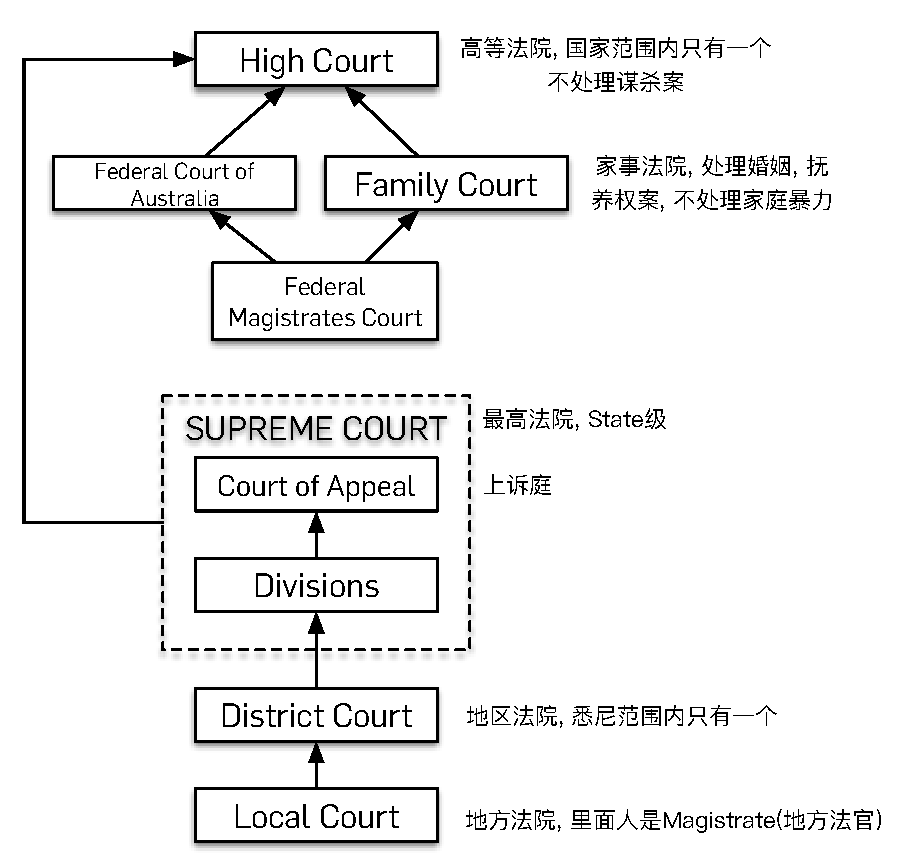
\includegraphics{pics/court.pdf}
\end{figure}

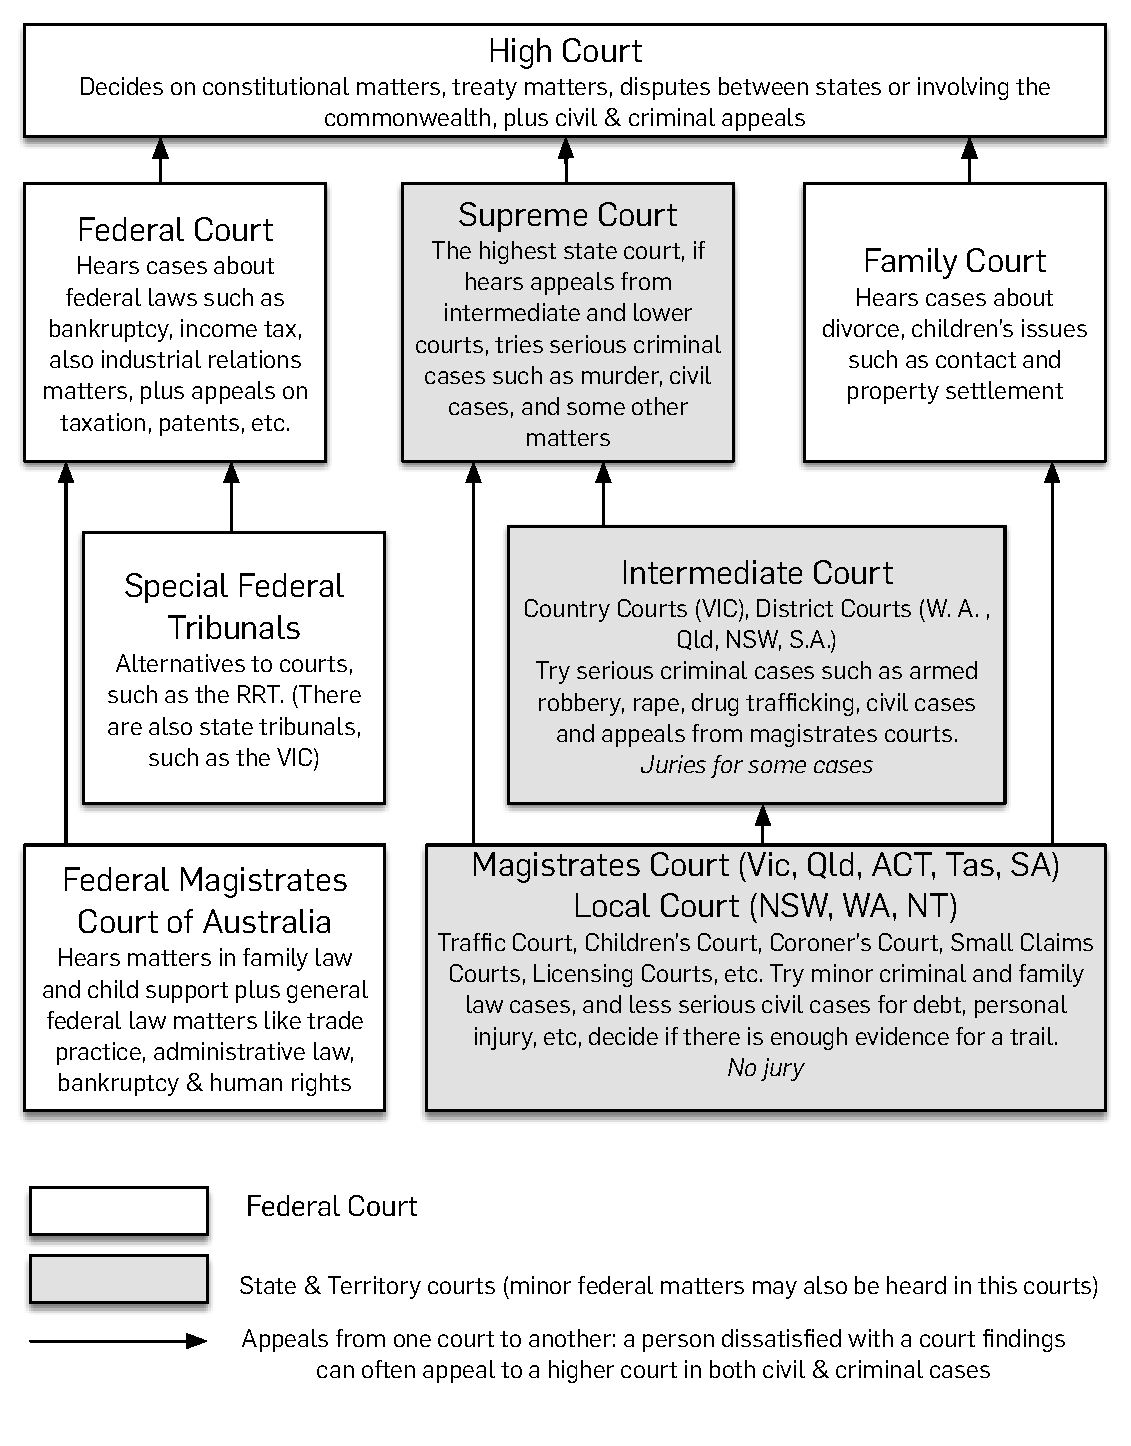
\includepdf[pages={-}]{pics/court2.pdf}

\section{澳大利亞地方法院介紹}
Most courts in Australia have a similar layout. The picture below shows the layout of a Magistrate’s Court in South Australia. Around 90\% of all court cases begin and end in a Magistrate’s Court. It is a busy court. Apart from differences in size and decor, higher courts such as the District Court and Supreme Court hearing criminal cases have a space for a jury.

In many higher courts, there is a physical separation between those facing the gallery, those presenting information in court (the Bar Table is where those presenting information or evidence to the court sit and stand) and the Bench where the Magistrate sits. The space between these is often called the `well' and tradition has it that nothing should pass through that space when court is in session except the truth.

\begin{center}
    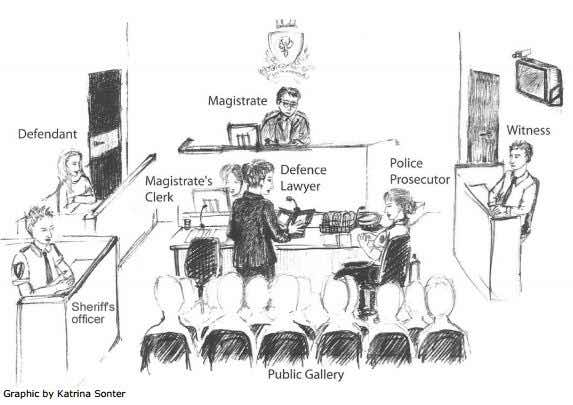
\includegraphics[scale=.8]{pics/magistrate-court}
\end{center}

\begin{itemize}
  \itemsep0em
  \item Magistrate: Magistrates are lawyers who have worked for at least five years. A magistrate hears evidence and decides whether a person is guilty or not guilty to an offence as charged. A magistrate imposes a penalty on those who are either found guilty or plead guilty to offences. The magistrate's role in court is to ensure that justice is administered fairly and impartially. Magistrates usually dress in business clothing but some now choose to wear a black robe without a wig.
  \item Magistrate's clerk: The magistrate's clerk ensures that a proper record of the proceedings of the court is maintained. The clerk records the evidence presented to the court, the magistrate's remarks, decisions and penalties.
  \item Defendant: The defendant, also known as the accused, is the person who has allegedly committed a crime. The defendant may represent him/herself but most people hire a lawyer to represent them. Those that fit certain criteria may be able to seek legal aid.
  \item Counsel: Generally speaking, the word ‘counsel’ describes lawyers who prosecute (or claim if it is in a civil suit) and defend (or respond in civil cases). They are officers of the Court and provide ‘counsel’ or advice to the Magistrate about the law and the case. The defence counsel’s job is to defend the person who is accused of committing a crime. This is done by challenging the prosecution, cross examining witnesses for the prosecution, providing witnesses for the defence and any information that establishes reasonable doubt about the truth of the prosecution allegation.
  \item Prosecutor: The State prosecutes a person for a crime. The prosecutor can be an individual representing the State, such as a Police Prosecutor or a Public Prosecutor who works for the Office of the Director of Public Prosecutions; a representative of a State or Government department (for example, a park ranger, fisheries officer); a Local Government Council (for example, a council health inspector or a council planning inspector); or a private individual. The prosecutor is not necessarily a lawyer.  It is the prosecutor's job to provide the court with information as to the type of offence the defendant is alleged to have committed and prove beyond reasonable doubt that the defendant committed the crime as charged.
  \item Witness: The prosecution and defence may call witnesses to present information about what they may have seen or heard. The witness may also corroborate other information.
  \item Sheriff's Officer: There is only one Sheriff in South Australia but the Sheriff has more than 100 officers. Sheriff’s Officers keep order in the court, help to bring prisoners into and out of court, and help people coming into the courtroom. They advise the magistrate's clerk as to which defendants, solicitors and so on are present in court and if they are ready to proceed with their case. They make sure defendants do not leave court without signing any bonds, bails or orders of the court if that is what is required. In a courthouse and associated property, a Sheriff’s Officer has the powers of the police to arrest a person who misbehaves.
\end{itemize}

\section{澳大利亞不同的仲裁庭}
\begin{itemize}
  \itemsep0em
  \item Administrative Appeals Tribunal (AAT): 行政事務上訴仲裁庭
  \item Civil and Administrative Tribunal (CAT): 民事與行政仲裁庭
  \item Copyright Tribunal of Australia: 澳大利亞版權(保護)上訴仲裁庭
  \item Consumer, Trader \& Tenancy Tribunal (CTTT): 消費者, 商家及租務仲裁庭
  \item Migration Review Tribunal (MRT): 移民復議仲裁庭
  \item Refugee Review Tribunal (RRT): 難民復議仲裁庭
  \item Social Security Appeals Tribunal (SSAT): 社會保障上訴仲裁庭
\end{itemize}

\begin{itemize}
  \itemsep0em
  \item 審訊 / 審判: trail / sentence
  \item 提堂 / 聽審: mention\footnote{問嫌疑人是否認罪} / hearing\footnote{基於不認罪的情況下進行}
\end{itemize}

\section{各種法律懲罰}
\begin{multicols}{2}
\begin{itemize}
  \itemsep0em
  \item 罰款: fine
  \item 社區服務令: Community Service Order\footnote{詳情:\url{http://www.judcom.nsw.gov.au/publications/benchbks/sentencing/community_service_orders.html}}
  \item 守行為保證: Good Behaviour Bond
  \item 緩刑 / 假釋 / 保釋: probation / parole ($v.$ + $n.$) / bail
  \item 週末服刑: Weekend jail
  \item 家中監禁: Home Detention
  \item 上繳: surrender (也可以指投降)
  \item 入獄: imprisonment / jail sentence
  \item 終身監禁: life sentence
  \item 死刑: death penalty
\end{itemize}
\end{multicols}

\section{和立遗嘱有关的词汇}
\begin{multicols}{2}
\begin{itemize}
  \itemsep0em
  \item 立遺囑: make a will
  \item 遺囑: last will / testament
  \item 立遺囑的人: testator
  \item 沒有立的遺囑: intestate ($n.$ + $adj.$, $adj.$一般作後置)
  \item 沒有遺囑的財產: intestate property
  \item 分財產: distribute / split assets (或property)
  \item 遺囑檢驗: probate ($n.$ + $adj.$ + $v.$)
  \item 遺囑執行人(男 / 女): executor / executrix
  \item 遺囑受益人: beneficiary
  \item 遺囑見證人: witness(一般用複數加es)
  \item 自助草擬遺囑工具包: DIY Will Kit
  \item 遺囑附錄: codicil
  \item 遺產 / 遺產稅: estate / estate tax
\end{itemize}
\end{multicols}

\section{各種打人的方式}
\begin{multicols}{2}
\begin{itemize}
  \itemsep0em
  \item 揍 / 抽: punch ($sb.$'s face) / slap (in the face)
  \item 踢 / 推 / 拉: kick / push / pull
  \item 抓 / 戳 / 掐: scratch / poke / pinch
  \item (用手肘)勒: elbow (當$v.$使用即可)
  \item 勒脖子: strangle $sb.$ by the neck
  \item 朝著某人開槍: shoot at $sb.$
  \item 他被槍射中了: He got shoot.
  \item 他\hilight{沒有}被槍射中: He got shoot at.
\end{itemize}
\end{multicols}